\chapter{Das Elman Netz}
Elman Netze\cite{elman} besitzen die Eigenschaft zeitver�nderliche Muster zu erkennen und zu klassifizieren, da bei einem Elman Netz der Output der verdeckten Schicht gespeichert und zeitversetzt als Input verwendet wird, indem man in der Inputschicht eine Kontextschicht anlegt.
\begin{figure}[H]
	\centering
	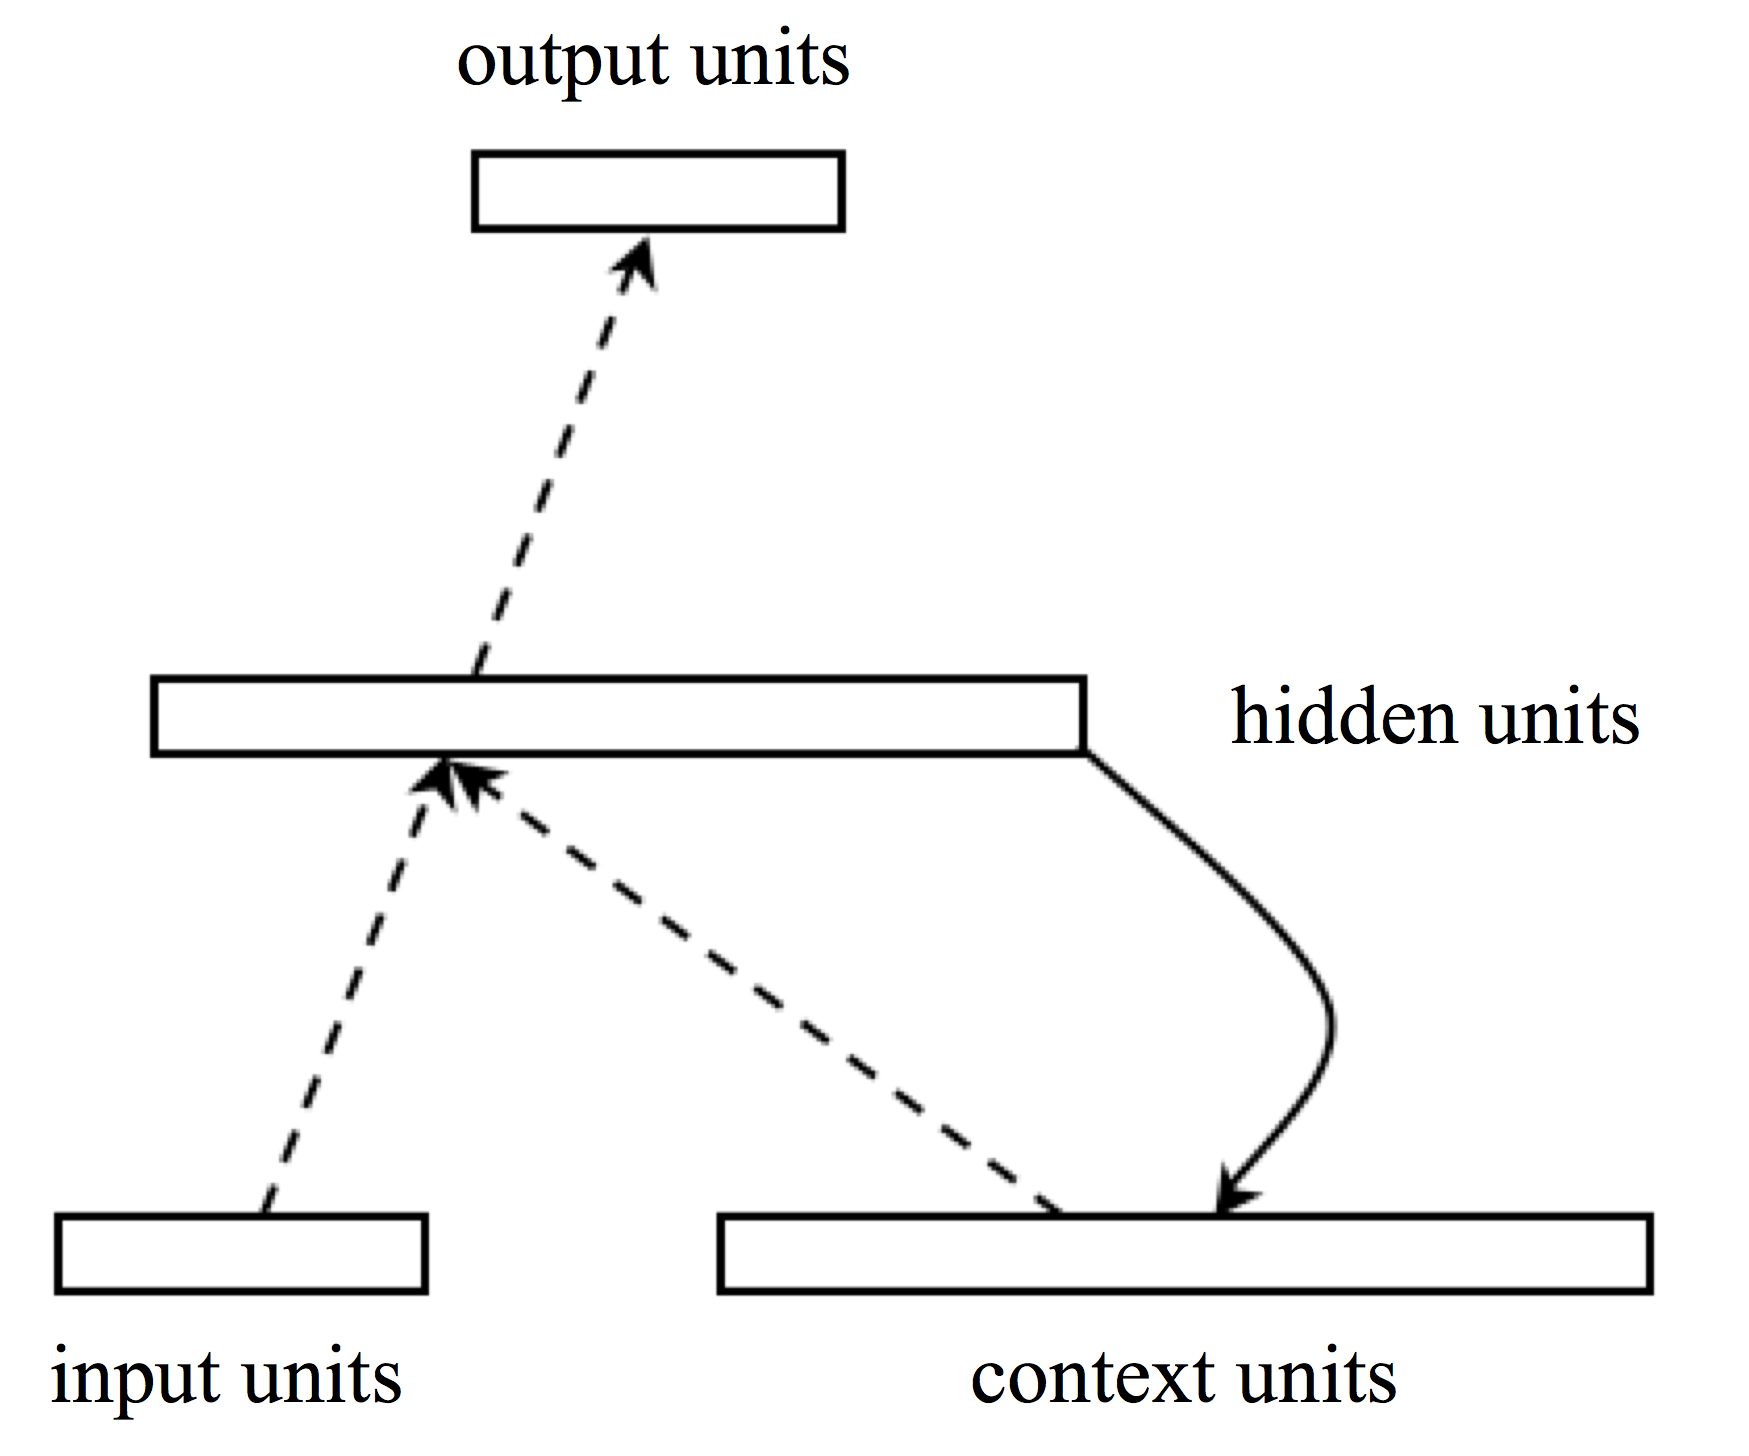
\includegraphics[height=6cm]{elman.png}
	\caption{Elman Network\itshape(plato.stanford.edu)\upshape}
	\label{elmanNet}
\end{figure}
Die Architektur (Abbildung \ref{elmanNet}) eines Elman Netzes besteht also aus einer Inputschicht, einer verdeckten Schicht, einer Outputschicht und der Kontextschicht, in der die Werte der verdeckten Schicht zeitversetzt gespeichert werden. Somit wird der innere Zustand des Netzes in der Kontextschicht gespeichert.